%Группа 11-1 Модуль 3
\cheadbf{Модуль 3 Занятие 2}
\begin{listofex}
	\item Вычислить:
	\begin{enumcols}[itemcolumns=3]
		\item \exercise{1665}
		\item \exercise{1775}
		\item \exercise{1221}
		\item \exercise{1578}
		\item \exercise{1589}
		\item \exercise{1137}
		\item \exercise{2984}
	\end{enumcols}
	\item Некоторая компания продает свою продукцию по цене\(  p=500  \)руб. за единицу, переменные затраты на производство одной единицы продукции составляют  \( v=300 \) руб., постоянные расходы предприятия \( f=700000 \) руб. в месяц. Месячная операционная прибыль предприятия (в рублях) вычисляется по формуле  \( \pi(q)=q(p-v)-f \). Определите месячный объeм производства\(  q \) (единиц продукции), при котором месячная операционная прибыль предприятия будет равна \( 300000 \) руб.
	\item Зависимость объёма спроса \( q \) (единиц в месяц) на продукцию предприятия – монополиста от цены \( p \) (тыс. руб.) задаётся формулой \( q=100-10p \). Выручка предприятия за месяц \( r \) (в тыс. руб.) вычисляется по формуле \( r(p)=q\cdot p \). Определите наибольшую цену \( p \), при которой месячная выручка \( r(p) \) составит не менее \( 240 \) тыс. руб. Ответ приведите в тыс. руб.
	\item По закону Ома для полной цепи сила тока, измеряемая в амперах, равна \( I=\dfrac{\sigma}{R+r} \), где \(\sigma\) – ЭДС источника (в вольтах), \(r=2\) Ом – его внутреннее сопротивление, \(R\) – сопротивление цепи (в омах). При каком наименьшем сопротивлении цепи сила тока будет составлять не более \(40\% \) от силы тока короткого замыкания \( I_{кз} =\dfrac{\sigma}{r}\)? (Ответ выразите в омах).
	\item Гоночный автомобиль разгоняется на прямолинейном участке шоссе с постоянным ускорением \( a \) км/ч\( ^2 \). Скорость \( v \)  в конце пути вычисляется по формуле \( v=\sqrt{2la} \), где \( l \) – пройденный автомобилем путь в км. Определите ускорение, с которым должен двигаться автомобиль, чтобы, проехав \( 250 \) метров, приобрести скорость \( 60 \)км/ч. Ответ выразите в км/ч\( ^2 \).
	\item Расстояние (в км) от наблюдателя, находящегося на небольшой высоте \( h \) километров над землeй, до наблюдаемой им линии горизонта вычисляется по формуле \( l=\sqrt{2Rh} \), где \( R = 6400 \) (км) – радиус Земли. С какой высоты горизонт виден на расстоянии \(4\) километра? Ответ выразите в километрах.
	\item Фабрика выпускает сумки. В среднем на \( 110 \) качественных сумок приходится одиннадцать сумок со скрытыми дефектами. Найдите вероятность того, что купленная сумка окажется качественной. Результат округлите до сотых.
	\item На борту самолёта \( 13 \) мест рядом с запасными выходами и \( 19 \) мест за перегородками, разделяющими салоны. Остальные места неудобны для пассажира высокого роста. Пассажир В. высокого роста. Найдите вероятность того, что на регистрации при случайном выборе места пассажиру В. достанется удобное место, если всего в самолёте \( 200 \) мест.
	\item Девять одинаковых рубашек дешевле куртки на \( 10\% \). На сколько процентов четырнадцать таких же рубашек дороже куртки?
	\item Игорь и Паша красят забор за \( 15 \) часов. Паша и Володя красят этот же забор за \( 21 \) час, а Володя и Игорь – за \( 35 \) часов. За сколько часов мальчики покрасят забор, работая втроем?
\end{listofex}
\newpage
\cheadbf{Модуль 3 Домашняя работа 1}
\begin{listofex}
	\item Вычислить:
	\begin{enumcols}[itemcolumns=3]
		\item \exercise{1689}
		\item \exercise{1776}
		\item \( \sqrt{7}\cdot\sqrt[4]{7}\cdot\sqrt[8]{7} \)
		\item \exercise{569}
		\item \exercise{588}
		\item \exercise{2994}
		\item \( 14\cos(-135\degree)\cdot\sin(-45\degree) \)
	\end{enumcols}
	\item При температуре \( 0^{\circ}  \) рельс имеет длину \( l_0=12,5 \)м. При возрастании температуры происходит тепловое расширение рельса, и его длина, выраженная в метрах, меняется по закону \( l(t^{\circ})=l_0(1+\alpha\cdot t^{\circ}) \), где  \( \alpha=1,2\cdot 10^{-5}(^{\circ}C)^{-1} \) – коэффициент теплового расширения, \( t^{\circ} \) – температура (в градусах Цельсия). При какой температуре рельс удлинится на \( 6 \) мм? Ответ выразите в градусах Цельсия.
	\item Некоторая компания продаёт свою продукцию по цене \( p = 600 \) руб. за единицу, переменные затраты на производство одной единицы продукции составляют \( v = 300 \) руб., постоянные расходы предприятия \( f = 700 000 \) руб. в месяц. Месячная операционная прибыль предприятия (в рублях) вычисляется по формуле \(g(q)=q(p-v)-f\). Определите месячный объём производства \( q \) (единиц продукции), при котором месячная операционная прибыль предприятия будет равна \( 500 000 \) руб.
	\item По закону Ома для полной цепи сила тока, измеряемая в амперах, равна \( I=\dfrac{\sigma}{R+r} \), где \(\sigma\) – ЭДС источника (в вольтах), \(r=4\) Ом – его внутреннее сопротивление, \(R\) – сопротивление цепи (в омах). При каком наименьшем сопротивлении цепи сила тока будет составлять не более \( 60\% \) от силы тока короткого замыкания \( I_{кз} =\dfrac{\sigma}{r}\)? (Ответ выразите в омах).
	\item На экзамен вынесено \( 60 \) вопросов, Андрей не выучил \( 3 \) из них. Найдите вероятность того, что ему попадется выученный вопрос.
	\item У Вити в копилке лежит \( 12 \) рублёвых, \( 6 \) двухрублёвых, \( 4 \) пятирублёвых и \( 3 \) десятирублёвых монеты. Витя наугад достаёт из копилки одну монету. Найдите вероятность того, что оставшаяся в копилке сумма составит более \( 70 \) рублей.
	\item Игорь и Паша красят забор за \( 21 \) час. Паша и Володя красят этот же забор за \( 28 \) часов, а Володя и Игорь – за \( 60 \) часов. За сколько часов мальчики покрасят забор, работая втроем?
	\item Четыре одинаковые рубашки дешевле куртки на \( 8\% \). На сколько процентов пять таких же рубашек дороже куртки?
	\item Решить уравнение:
	\begin{enumcols}[itemcolumns=2]
		\item \( \sqrt{\dfrac{1}{15x-4}}=0,2 \)
		\item \( \log_5(x^2+2x)=\log_5(x^2+10) \)
		\item \( \left( \dfrac{1}{3} \right)^{x-8}=\dfrac{1}{9} \)
	\end{enumcols}
\end{listofex}
\newpage
\cheadbf{Модуль 3 Занятие 3}
\begin{listofex}
	\item При изготовлении подшипников диаметром 67 мм вероятность того, что диаметр будет отличаться от заданного не больше, чем на 0,01 мм, равна 0,965. Найдите вероятность того, что случайный подшипник будет иметь диаметр меньше чем 66,99 мм или больше чем 67,01 мм.
	\item Вероятность того, что в случайный момент времени температура тела здорового человека окажется ниже чем 36,8 °С, равна 0,81. Найдите вероятность того, что в случайный момент времени у здорового человека температура окажется 36,8 °С или выше.
	\item Вероятность того, что батарейка бракованная, равна 0,06. Покупатель в магазине выбирает случайную упаковку, в которой две таких батарейки. Найдите вероятность того, что обе батарейки окажутся исправными.
	\item Если шахматист А. играет белыми фигурами, то он выигрывает у шахматиста Б. с вероятностью 0,52. Если А. играет черными, то А. выигрывает у Б. с вероятностью 0,3. Шахматисты А. и Б. играют две партии, причём во второй партии меняют цвет фигур. Найдите вероятность того, что А. выиграет оба раза.
	\item В магазине три продавца. Каждый из них занят обслуживанием клиента с вероятностью 0,2 независимо от других продавцов. Найдите вероятность того, что в случайный момент времени все три продавца заняты.
	\item В торговом центре два одинаковых автомата продают кофе. Обслуживание автоматов происходит по вечерам после закрытия центра. Известно, что вероятность события «К вечеру в первом автомате закончится кофе» равна 0,25. Такая же вероятность события «К вечеру во втором автомате закончится кофе». Вероятность того, что кофе к вечеру закончится в обоих автоматах, равна 0,15. Найдите вероятность того, что к вечеру дня кофе останется в обоих автоматах.
	\item Из районного центра в деревню ежедневно ходит автобус. Вероятность того, что в понедельник в автобусе окажется меньше 20 пассажиров, равна 0,94. Вероятность того, что окажется меньше 15 пассажиров, равна 0,56. Найдите вероятность того, что число пассажиров будет от 15 до 19.
	\item Вероятность того, что новый электрический чайник прослужит больше года, равна 0,97. Вероятность того, что он прослужит больше двух лет, равна 0,89. Найдите вероятность того, что он прослужит меньше двух лет, но больше года.
	\item Помещение освещается фонарём с двумя лампами. Вероятность перегорания лампы в течение года равна 0,3. Найдите вероятность того, что в течение года хотя бы одна лампа не перегорит.
	\item В Волшебной стране бывает два типа погоды: хорошая и отличная, причём погода, установившись утром, держится неизменной весь день. Известно, что с вероятностью 0,8 погода завтра будет такой же, как и сегодня. Сегодня 3 июля, погода в Волшебной стране хорошая. Найдите вероятность того, что 6 июля в Волшебной стране будет отличная погода.
	\item Ковбой Джон попадает в муху на стене с вероятностью 0,9, если стреляет из пристрелянного револьвера. Если Джон стреляет из непристрелянного револьвера, то он попадает в муху с вероятностью 0,2. На столе лежит 10 револьверов, из них только 4 пристрелянные. Ковбой Джон видит на стене муху, наудачу хватает первый попавшийся револьвер и стреляет в муху. Найдите вероятность того, что Джон промахнётся.
\end{listofex}
%\newpage
%\title{Занятие №4}
%\begin{listofex}
%	
%\end{listofex}
\newpage
\cheadbf{Модуль 3 Домашняя работа 2}
\begin{listofex}
	\item После дождя уровень воды в колодце может повыситься. Мальчик измеряет время \( t \) падения небольших камешков в колодец и рассчитывает расстояние до воды по формуле \( h=5t^2 \), где \( h \) - расстояние в метрах, \( t \) а - время падения в секундах. До дождя время падения камешков составляло \( 0,6 \) с. На сколько должен подняться уровень воды после дождя, чтобы измеряемое время изменилось на \( 0,2 \) с? Ответ выразите в метрах.
	\item Для нагревательного элемента некоторого прибора экспериментально была получена зависимость температуры (в кельвинах) от времени работы: \( T(t) = T_0 + bt + at^2 \), где \( t \) - время в минутах, \( T_0 = 1400 \) К, \( a = -10 \) К/мин$^{2}$, \( b = 200 \) К/мин. Известно, что при температуре нагревателя свыше \( 1760 \) К прибор может испортиться, поэтому его нужно отключить. Определите, через какое наибольшее время после начала работы нужно отключить прибор. Ответ выразите в минутах.
	\item Скейтбордист прыгает на стоящую на рельсах платформу, со скоростью \(u = 3\)  м/с под острым углом \(a\) к рельсам. От толчка платформа начинает ехать со скоростью \(u = \dfrac{m}{m+M}\cdot v\cdot cos{a}\)  (м/с), где \(m = 80\) кг — масса скейтбордиста со скейтом, а \(M = 400\) кг — масса платформы. Под каким максимальным углом \(a\)  (в градусах) нужно прыгать, чтобы разогнать платформу не менее чем до \(0,25\) м/с?
	\item Некоторая компания продает свою продукцию по цене \(  p=2000  \)руб. за единицу, переменные затраты на производство одной единицы продукции составляют  \( v=1100 \) руб., постоянные расходы предприятия \( f=600000 \) руб. в месяц. Месячная операционная прибыль предприятия (в рублях) вычисляется по формуле  \( \pi(q)=q(p-v)-f \). Определите месячный объeм производства\(  q \) (единиц продукции), при котором месячная операционная прибыль предприятия будет равна \( 300000 \) руб.
	\item Велосипедист выехал с постоянной скоростью из города \(A\) в город \(B\), расстояние между которыми равно \(70\) км. На следующий день он отправился обратно в \(A\) со скоростью на \(3\) км/ч больше прежней. По дороге он сделал остановку на \(3\) часа. В результате велосипедист затратил на обратный путь столько же времени, сколько на путь из \(A\) в \(B\). Найдите скорость велосипедиста на пути из \(B\) в \(A\). Ответ дайте в км/ч.
	\item Два гонщика участвуют в гонках. Им предстоит проехать 60 кругов по кольцевой трассе протяжённостью \(3\) км. Оба гонщика стартовали одновременно, а на финиш первый пришёл раньше второго на \(10\) минут. Чему равнялась средняя скорость второго гонщика, если известно, что первый гонщик в первый раз обогнал второго на круг через \(15\) минут? Ответ дайте в км/ч.
	\item Первая труба пропускает на \(1\) литр воды в минуту меньше, чем вторая. Сколько литров воды в минуту пропускает первая труба, если резервуар объемом \(110\) литров она заполняет на \(2\) минуты дольше, чем вторая труба заполняет резервуар объемом \(99\) литров?
	\item Две бригады, состоящие из рабочих одинаковой квалификации, одновременно начали выполнять два одинаковых заказа. В первой бригаде было \(16\) рабочих, а во второй — \(25\) рабочих. Через \(7\) дней после начала работы в первую бригаду перешли \(8\) рабочих из второй бригады. В итоге оба заказа были выполнены одновременно. Найдите, сколько дней потребовалось на выполнение заказов.
	\newpage
	\item Решите уравнения:
	\begin{enumcols}[itemcolumns=2]
		\item \( \sqrt{\dfrac{6}{4x-54}}=\dfrac{1}{7} \)
		\item \( \sqrt{\dfrac{2x+5}{3}}=5 \)
		\item \( \log_82^{8x-4}=4 \)
		\item \( \log_{x-4}32=5 \)
		\item \( 8^{9-x}=64^x\)
		\item \( 9^{-5+x}=729 \)
	\end{enumcols}
	\item Вычислить:
	\begin{enumcols}[itemcolumns=1]
		\item \exercise{1116}
		\item \exercise{1118}
	\end{enumcols}
	\item \begin{minipage}[t]{0.66\textwidth}
		На рисунке изображены графики функций \( f(x)=-4x+9 \) и \( g(x)=ax^2+bx+c \), которые пересекаются в точках \(A\) и \(B\). Найдите абсциссу  \( B \).
	\end{minipage}
	\begin{minipage}[c]{0.3\textwidth}
		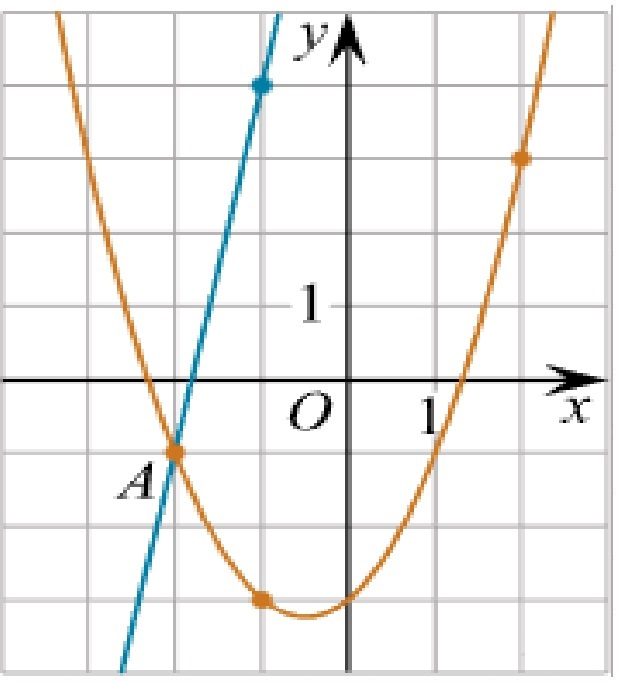
\includegraphics[align=b, width=0.8\textwidth]{pics/G111M3H2-1}
	\end{minipage}
\end{listofex}
%\newpage
%\title{Занятие №5}
%\begin{listofex}
%	
%\end{listofex}
%\newpage
%\title{Занятие №6}
%\begin{listofex}
%	
%\end{listofex}
%\newpage
%\title{Домашняя работа №3}
%\begin{listofex}
%	
%\end{listofex}
\newpage
\cheadbf{Подготовка к проверочной работе}
\begin{listofex}
	\item Вычислить:
	\begin{enumcols}[itemcolumns=2]
		\item \exercise{1667}
		\item \exercise{1772}
		\item \exercise{1770}
		\item \exercise{1570}
		\item \exercise{1575}
		\item \exercise{1588}
	\end{enumcols}
	\item Расстояние (в км) от наблюдателя, находящегося на небольшой высоте \( h \) километров над землeй, до наблюдаемой им линии горизонта вычисляется по формуле \( l=\sqrt{2Rh} \), где \( R = 6400 \) (км) – радиус Земли. С какой высоты горизонт виден на расстоянии \(4\) километра? Ответ выразите в километрах.
	\item При температуре \( 0^{\circ}  \) рельс имеет длину \( l_0=12,5 \)м. При возрастании температуры происходит тепловое расширение рельса, и его длина, выраженная в метрах, меняется по закону \( l(t^{\circ})=l_0(1+\alpha\cdot t^{\circ}) \), где  \( \alpha=1,2\cdot 10^{-5}(^{\circ}C)^{-1} \) – коэффициент теплового расширения, \( t^{\circ} \) – температура (в градусах Цельсия). При какой температуре рельс удлинится на \( 6 \) мм? Ответ выразите в градусах Цельсия.
	\item По закону Ома для полной цепи сила тока, измеряемая в амперах, равна \( I=\dfrac{\sigma}{R+r} \), где \(\sigma\) – ЭДС источника (в вольтах), \(r=2\) Ом – его внутреннее сопротивление, \(R\) – сопротивление цепи (в омах). При каком наименьшем сопротивлении цепи сила тока будет составлять не более \(40\% \) от силы тока короткого замыкания \( I_{кз} =\dfrac{\sigma}{r}\)? (Ответ выразите в омах).
	\item Фабрика выпускает сумки. В среднем на \( 150 \) качественных сумок приходится тридцать сумок со скрытыми дефектами. Найдите вероятность того, что купленная сумка окажется качественной. Результат округлите до сотых.
	\item На экзамен вынесено \( 120 \) вопросов, Андрей не выучил \( 6 \) из них. Найдите вероятность того, что ему попадется выученный вопрос.
	\item Из районного центра в деревню ежедневно ходит автобус. Вероятность того, что в понедельник в автобусе окажется меньше 20 пассажиров, равна 0,94. Вероятность того, что окажется меньше 15 пассажиров, равна 0,56. Найдите вероятность того, что число пассажиров будет от 15 до 19.
	\item Первая труба пропускает на \(1\) литр воды в минуту меньше, чем вторая. Сколько литров воды в минуту пропускает первая труба, если резервуар объемом \(110\) литров она заполняет на \(2\) минуты дольше, чем вторая труба заполняет резервуар объемом \(99\) литров?
	\item Два гонщика участвуют в гонках. Им предстоит проехать \(68\) кругов по кольцевой трассе протяжённостью \(6\) км. Оба гонщика стартовали одновременно, а на финиш первый пришёл раньше второго на \(15\) минут. Чему равнялась средняя скорость второго гонщика, если известно, что первый гонщик в первый раз обогнал второго на круг через \(60\) минут? Ответ дайте в км/ч.
	\item Решить уравнение:
	\begin{enumcols}[itemcolumns=2]
		\item \( \sqrt{\dfrac{1}{x}}=0,2 \)
		\item \( \left( \dfrac{1}{3} \right)^{x}=27 \)
		\item \( \log_5(x^2+2x)=\log_{5}(x^2+6x+4) \)
		\item \( \log_5(x^2+2x-10)=\sqrt[]{25} \)
	\end{enumcols}
	\item Вычислить:
	\begin{enumcols}[itemcolumns=1]
		\item \exercise{1117}
		\item \exercise{1119}
	\end{enumcols}
	\item Вычислить:
	\begin{enumcols}[itemcolumns=2]
		\item \(\dfrac{24(\sin^2{17\degree}-\cos^2{17\degree})}{\cos{34\degree}} \)
		\item \(4 \cdot \sqrt[]{2} \cos{\dfrac{\pi}{4}} \cos{\dfrac{7\pi}{3}} \)
		\item \(\dfrac{28}{\sin{\dfrac{-25\pi}{4}}\cos{\dfrac{23\pi}{4}}} \)
		\item \(\dfrac{4\cos{146\degree}}{\cos{34\degree}} \)
		\item \(\dfrac{6}{\cos^2{23\degree}+\cos^2{113\degree}} \)
		\item \(\dfrac{50\sin{19\degree} \cdot \cos{19\degree}}{\sin{38\degree}} \)
	\end{enumcols}
	\item \begin{minipage}[t]{0.66\textwidth}
		На рисунке изображены графики функций \( f(x)=4x^2-25x+41 \) и \( g(x)=ax^2+bx+c \), которые пересекаются в точках \(A\) и \(B\). Найдите абсциссу  \( B \).
	\end{minipage}
	\begin{minipage}[c]{0.3\textwidth}
		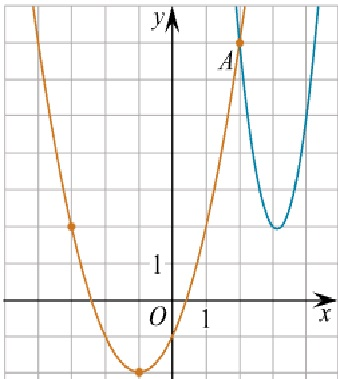
\includegraphics[align=b, width=0.8\textwidth]{pics/G111M3PP-1}
	\end{minipage}
	\item \begin{minipage}[t]{0.66\textwidth}
		На рисунке изображены графики двух линейных функций. Найдите абсциссу точки пересечения графиков.
	\end{minipage}
	\begin{minipage}[c]{0.3\textwidth}
		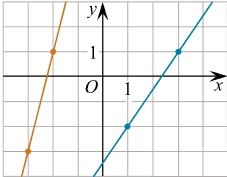
\includegraphics[align=b, width=0.8\textwidth]{pics/G111M3PP-2}
	\end{minipage}
\end{listofex}
\newpage
\cheadbf{Проверочная работа}
\begin{listofex}
	\item Вычислить:
	\begin{enumcols}[itemcolumns=2]
		\item \exercise{1660}
		\item \exercise{1775}
		\item \exercise{1759}
		\item \exercise{1588}
		\item \exercise{1574}
		\item \exercise{1576}
	\end{enumcols}
	\item Решить уравнение:
	\begin{enumcols}[itemcolumns=2]
		\item \( \sqrt{\dfrac{200}{x+11}}=10 \)
		\item \( \sqrt{\dfrac{5}{125(x-4)}}=0,2 \)
		\item \( \left( \dfrac{1}{4} \right)^{x}=256 \)
		\item \(  3^{x}=\left( \dfrac{1}{9} \right)^{-2} \)
		\item \( \log_6(x^2+2x+1)=2 \)
		\item \( \log_3(4x^2-5x+32)=\log_9(3x^2-5x+17) \)
	\end{enumcols}
	\item Вычислить:
	\begin{enumcols}[itemcolumns=2]
		\item \(\dfrac{\cos{31\degree}}{\cos{149\degree}} \)
		\item \(\sqrt[]{2} \cos{\dfrac{3\pi}{4}} \cos{\dfrac{5\pi}{3}} \)
		\item \(\dfrac{24(\sin^2{35\degree}-\cos^2{35\degree})}{\cos{70\degree}} \)
		\item \(\dfrac{0,5}{\sin{\dfrac{-15\pi}{4}}\cos{\dfrac{33\pi}{4}}} \)
	\end{enumcols}
	\item Вычислить:
	\begin{enumcols}[itemcolumns=1]
		\item \( \cos\left(a+{\dfrac{3\pi}{2}}\right) \), если \( \cos{a} = -0,6 \) и \(a \in \left( \pi;\dfrac{3\pi}{2} \right) \)
		\item \( \sin\left({\dfrac{7\pi}{2}-a}\right) \), если \( \sin{a} = 0,8 \) и \(a\in\left( \dfrac{\pi}{2};\pi \right) \)
		\item \( \tg{a},\) если \( \cos{a} = \dfrac{\sqrt{10}}{10} \) и \(a\in\left( \dfrac{3\pi}{2};2\pi \right) \)
	\end{enumcols}
	\item Груз массой \(0,08\) кг колеблется на пружине. Его скорость \(v\) меняется по закону \( v = v_0 \cos{\dfrac{2\pi t}{T}}\), где \(t\) — время с момента начала колебаний, \(T = 2\) с — период колебаний, \(v_0=0,5\) м/с. Кинетическая энергия \(E\) (в джоулях) груза вычисляется по формуле \(E=\dfrac{mv^2}{2}\), где \(m\) — масса груза в килограммах, \(v\) — скорость груза в м/с. Найдите кинетическую энергию груза через \(1\) секунду после начала колебаний. Ответ дайте в джоулях.
	\item Зависимость объёма спроса \( q \) (единиц в месяц) на продукцию предприятия – монополиста от цены \( p \) (тыс. руб.) задаётся формулой \( q=100-10p \). Выручка предприятия за месяц \( r \) (в тыс. руб.) вычисляется по формуле \( r(p)=q\cdot p \). Определите наибольшую цену \( p \), при которой месячная выручка \( r(p) \) составит не менее \( 240 \) тыс. руб. Ответ приведите в тыс. руб.
	\item При производстве в среднем на каждые \(2982\) исправных насоса приходится \(18\) неисправных. Найдите вероятность того, что случайно выбранный насос окажется неисправным.
	\item На рок-фестивале выступают группы — по одной от каждой из заявленных стран. Порядок выступления определяется жребием. Какова вероятность того, что группа из Дании будет выступать после группы из Швеции и после группы из Норвегии? Результат округлите до сотых.
	\item Теплоход проходит по течению реки до пункта назначения \(200\) км и после стоянки возвращается в пункт отправления. Найдите скорость течения, если скорость теплохода в неподвижной воде равна \(15\) км/ч, стоянка длится \(10\) часов, а в пункт отправления теплоход возвращается через \(40\) часов после отплытия из него. Ответ дайте в км/ч.
	\item На изготовление \(475\) деталей первый рабочий тратит на \(6\) часов меньше, чем второй рабочий на изготовление \(550\) таких же деталей. Известно, что первый рабочий за час делает на \(3\) детали больше, чем второй. Сколько деталей в час делает первый рабочий?
	\item \begin{minipage}[t]{0.66\textwidth}
		На рисунке изображены графики двух линейных функций. Найдите абсциссу точки пересечения графиков.
	\end{minipage}
	\begin{minipage}[c]{0.3\textwidth}
		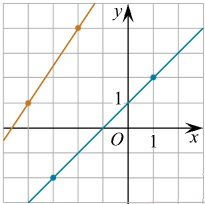
\includegraphics[align=b, width=0.8\textwidth]{pics/G111M3E-1}
	\end{minipage}
	\item \begin{minipage}[t]{0.66\textwidth}
		На рисунке изображены графики функций \( f(x)=4x^2+17x+14 \) и \( g(x)=ax^2+bx+c \), которые пересекаются в точках \(A\) и \(B\). Найдите абсциссу  \( B \).
	\end{minipage}
	\begin{minipage}[c]{0.3\textwidth}
		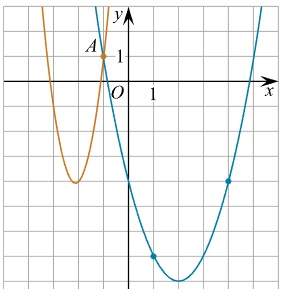
\includegraphics[align=b, width=0.8\textwidth]{pics/G111M3E-2}
	\end{minipage}
\end{listofex}
%\newpage
%\title{Проверочная работа}
%\begin{listofex}
%	
%\end{listofex}